\documentclass[dvisvgm]{standalone}
\usepackage{tikz}
\usepackage{pgfplots}
\pgfplotsset{compat=1.18}

\begin{document}
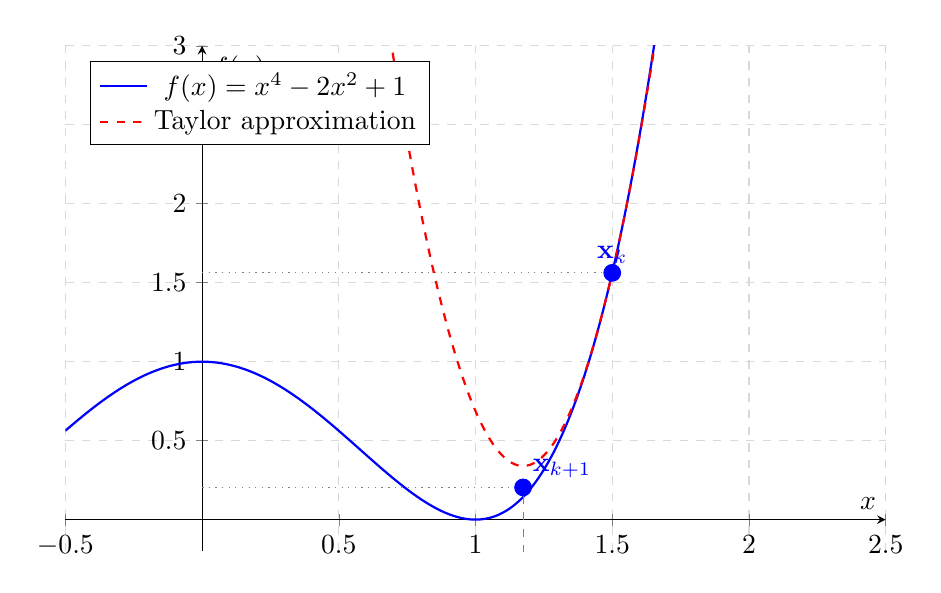
\begin{tikzpicture}
\begin{axis}[
    width=12cm,
    height=8cm,
    xmin=-0.5,
    xmax=2.5,
    ymin=-0.2,
    ymax=3,
    xlabel={$x$},
    ylabel={$f(x)$},
    grid=major,
    grid style={dashed, gray!30},
    axis lines=center,
    samples=200,
    smooth,
    legend pos=north west,
]

% Define the function f(x) = x^4 - 2x^2 + 1 (quartic with minimum at x=0)
% Starting point x_k = 1.5
% f(1.5) = 1.5625, f'(1.5) = 7.5, f''(1.5) = 23
% x_{k+1} = 1.5 - 7.5/23 ≈ 1.174

% Original function
\addplot[blue, thick, domain=-0.5:2.5] {x^4 - 2*x^2 + 1};
\addlegendentry{$f(x) = x^4 - 2x^2 + 1$}

% Second-order Taylor approximation around x_k = 1.5
% T(x) = f(x_k) + f'(x_k)(x-x_k) + (1/2)f''(x_k)(x-x_k)^2
% T(x) = 1.5625 + 7.5(x-1.5) + 11.5(x-1.5)^2
\addplot[red, thick, dashed, domain=0.5:2.5] {1.5625 + 7.5*(x-1.5) + 11.5*(x-1.5)^2};
\addlegendentry{Taylor approximation}

% Mark the starting point x_k on the curve
\addplot[only marks, mark=*, mark size=3pt, blue] coordinates {(1.5, 1.5625)};
\node[above, blue] at (axis cs:1.5, 1.5625) {$\mathbf{x}_k$};

% Mark the new point x_{k+1} on the curve
\addplot[only marks, mark=*, mark size=3pt, blue] coordinates {(1.174, 0.2039)};
\node[above right, blue] at (axis cs:1.174, 0.2039) {$\mathbf{x}_{k+1}$};

% Mark the minimum of the Taylor approximation
\addplot[only marks, mark=*, mark size=2pt, red] coordinates {(1.174, -1.056)};

% Draw vertical line from Taylor minimum to the curve
\addplot[gray, thin, dashed] coordinates {(1.174, -1.056) (1.174, 0.2039)};

% Draw horizontal line to show the x-coordinate
\addplot[gray, thin, dotted] coordinates {(0, 0.2039) (1.174, 0.2039)};
\addplot[gray, thin, dotted] coordinates {(0, 1.5625) (1.5, 1.5625)};

\end{axis}
\end{tikzpicture}
\end{document}
